%%  ************    LibreSilicon's 1st TestWafer    *******************
%%
%%  Organisation:   Chipforge
%%                  Germany / European Union
%%
%%  Profile:        Chipforge focus on fine System-on-Chip Cores in
%%                  Verilog HDL Code which are easy understandable and
%%                  adjustable. For further information see
%%                          www.chipforge.org
%%                  there are projects from small cores up to PCBs, too.
%%
%%  File:           PearlRiver/Documents/LaTeX/considerations.tex
%%
%%  Purpose:        Chapter File for Considerations
%%
%%  ************    LaTeX with circdia.sty package      ***************
%%
%%  ///////////////////////////////////////////////////////////////////
%%
%%  Copyright (c) 2018 by chipforge <hsank@nospam.chipforge.org>
%%  All rights reserved.
%%
%%      This Standard Cell Library is licensed under the Libre Silicon
%%      public license; you can redistribute it and/or modify it under
%%      the terms of the Libre Silicon public license as published by
%%      the Libre Silicon alliance, either version 1 of the License, or
%%      (at your option) any later version.
%%
%%      This design is distributed in the hope that it will be useful,
%%      but WITHOUT ANY WARRANTY; without even the implied warranty of
%%      MERCHANTABILITY or FITNESS FOR A PARTICULAR PURPOSE.
%%      See the Libre Silicon Public License for more details.
%%
%%  ///////////////////////////////////////////////////////////////////
\section{Considerations}

PearlRiver is the first Testwafer for the LibreSilicon 1 $ \mu m$ Technology.

This Testwafer should contain almost all test structures to evaulate and qualify the technology-depended paramters. So on Wafer we placed structures to measure the sheet-resistance of all Poly- and Metallayer, as well capacitors, NMOS and PMOS transistors, bipolar junction transistors, diodes and flash cells. There are even gate cells like NAND3, NOR3 and some others used for ring oscillators.

The parameter, measured from all test structures are used for the Spice3f and other models.


\subsection{Orientation}

There are to different systems to give orientation while talking about locations on the die. One systems use words like top (= upper side), right, buttion (= lower side) and left. The other systems uses cardinal directions like north, east, south and west to name the same. Both systems are very common, but here we use the cardinal directions, just as convention.

Wafers smaller than 8 inches, or 200 mm, have a flat side to give orientation and encode the crystal structure. Well, we like to call the side South with the notch or the flats.

All machines in the process flow has effects while dealing with the structures on the wafer. For instance etching is slightly more aggressiv on the eastern side of a structure than on the western side. To understand und measure this effects, all structures on the die are placed in a dedicated way. Structures are grouped together in a triangle. This triangle we call quarter, while placed four times on the same die, each rotated 90 degrees.

%%  ************    LibreSilicon's 1st TestWafer    *******************
%%
%%  Organisation:   Chipforge
%%                  Germany / European Union
%%
%%  Profile:        Chipforge focus on fine System-on-Chip Cores in
%%                  Verilog HDL Code which are easy understandable and
%%                  adjustable. For further information see
%%                          www.chipforge.org
%%                  there are projects from small cores up to PCBs, too.
%%
%%  File:           PearlRiver/Documents/LaTeX/die_quarter.tex
%%
%%  Purpose:        Principle Description Pictgure for quarters
%%
%%  ************    LaTeX with circdia.sty package      ***************
%%
%%  ///////////////////////////////////////////////////////////////////
%%
%%  Copyright (c) 2018 by chipforge <hsank@nospam.chipforge.org>
%%  All rights reserved.
%%
%%      This Standard Cell Library is licensed under the Libre Silicon
%%      public license; you can redistribute it and/or modify it under
%%      the terms of the Libre Silicon public license as published by
%%      the Libre Silicon alliance, either version 1 of the License, or
%%      (at your option) any later version.
%%
%%      This design is distributed in the hope that it will be useful,
%%      but WITHOUT ANY WARRANTY; without even the implied warranty of
%%      MERCHANTABILITY or FITNESS FOR A PARTICULAR PURPOSE.
%%      See the Libre Silicon Public License for more details.
%%
%%  ///////////////////////////////////////////////////////////////////
\begin{center}
    Principle - One Die with all Quarters
    \begin{figure}[h]
        \begin{center}
            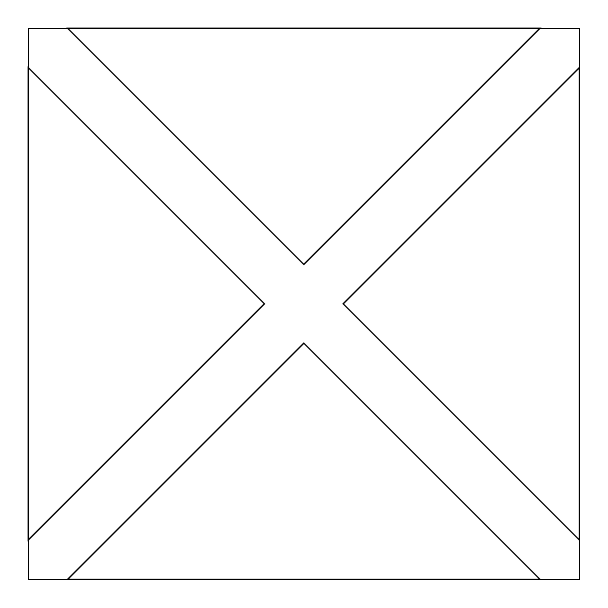
\begin{tikzpicture}[]
            \draw (0,0) -- (7,0) -- (7,7) -- (0,7) -- cycle;
            \draw (0.5,0) -- (6.5,0) -- (3.5,3) -- cycle;
            \draw (7,0.5) -- (7,6.5) -- (4,3.5) -- cycle;
            \draw (6.5,7) -- (0.5,7) -- (3.5,4) -- cycle;
            \draw (0,6.5) -- (0,0.5) -- (3,3.5) -- cycle;
            \end{tikzpicture}
        \end{center}
    \end{figure}
\end{center}


\subsection{Four-terminal Sensing}

%%  ************    LibreSilicon's 1st TestWafer    *******************
%%
%%  Organisation:   Chipforge
%%                  Germany / European Union
%%
%%  Profile:        Chipforge focus on fine System-on-Chip Cores in
%%                  Verilog HDL Code which are easy understandable and
%%                  adjustable. For further information see
%%                          www.chipforge.org
%%                  there are projects from small cores up to PCBs, too.
%%
%%  File:           PearlRiver/Documents/LaTeX/schematic_4terminal.tex
%%
%%  Purpose:        Schematic File for Four-terminal Sensing
%%
%%  ************    LaTeX with circdia.sty package      ***************
%%
%%  ///////////////////////////////////////////////////////////////////
%%
%%  Copyright (c) 2018 by chipforge <hsank@nospam.chipforge.org>
%%  All rights reserved.
%%
%%      This Standard Cell Library is licensed under the Libre Silicon
%%      public license; you can redistribute it and/or modify it under
%%      the terms of the Libre Silicon public license as published by
%%      the Libre Silicon alliance, either version 1 of the License, or
%%      (at your option) any later version.
%%
%%      This design is distributed in the hope that it will be useful,
%%      but WITHOUT ANY WARRANTY; without even the implied warranty of
%%      MERCHANTABILITY or FITNESS FOR A PARTICULAR PURPOSE.
%%      See the Libre Silicon Public License for more details.
%%
%%  ///////////////////////////////////////////////////////////////////
\begin{center}
    Schematic (Four-terminal Sensing)
    \begin{figure}[h]
        \begin{center}
            \begin{circuitdiagram}{32}{25}
            % current source with ground
            \ground{3}{0}{D}
            \wire{3}{1}{3}{8}
            \othersrc[\modify{RU}]{oo}{3}{11}{V}{}{}
            \wire{3}{14}{3}{21}
            % vertical flow, ampere meter
            \wire{3}{21}{12}{21}
            \measdev[\measunit{A}]{15}{21}{H}{$I_{drive}$}{}
            \wire{18}{21}{24}{21}
            \currarrow{20}{21}{R}{I}
            % pin contact
            \pin[\female]{25}{21}{R}{}
            \pin[\male]{25}{21}{L}{}
            %
            \pin[\female]{25}{1}{R}{}
            \pin[\male]{25}{1}{L}{}
            \ground{24}{0}{D}
            %
            \pin[\female]{25}{6}{R}{}
            \pin[\male]{25}{6}{L}{}
            %
            \pin[\female]{25}{16}{R}{}
            \pin[\male]{25}{16}{L}{}
            % voltage measurement
            \wire{15}{14}{15}{16}
            \wire{15}{16}{24}{16}
            \measdev[\measunit{V}]{15}{11}{V}{$V_{meas}$}{}
            \wire{15}{6}{15}{8}
            \wire{15}{6}{24}{6}
            \Voltarrow{25}{16}{25}{6}{r}{U}
            % device under test
            \resis{31}{11}{V}{device-under-test}{}
            \wire{26}{1}{30.5}{1}
            \pin{31}{1}{Dr}{I-}
            \wire{26}{6}{30.5}{6}
            \pin{31}{6}{UD}{U-}
            \wire{26}{16}{30.5}{16}
            \pin{31}{16}{UD}{U+}
            \wire{26}{21}{30.5}{21}
            \pin{31}{21}{Ur}{I+}
            %
            \wire{31}{2}{31}{5}
            \wire{31}{7}{31}{8}
            \wire{31}{14}{31}{15}
            \wire{31}{17}{31}{20}
            \end{circuitdiagram}
        \end{center}
    \end{figure}
\end{center}

%%  ************    LibreSilicon's 1st TestWafer    *******************
%%
%%  Organisation:   Chipforge
%%                  Germany / European Union
%%
%%  Profile:        Chipforge focus on fine System-on-Chip Cores in
%%                  Verilog HDL Code which are easy understandable and
%%                  adjustable. For further information see
%%                          www.chipforge.org
%%                  there are projects from small cores up to PCBs, too.
%%
%%  File:           PearlRiver/Documents/LaTeX/die_quarter.tex
%%
%%  Purpose:        Principle Description Pictgure for quarters
%%
%%  ************    LaTeX with circdia.sty package      ***************
%%
%%  ///////////////////////////////////////////////////////////////////
%%
%%  Copyright (c) 2018 by chipforge <hsank@nospam.chipforge.org>
%%  All rights reserved.
%%
%%      This Standard Cell Library is licensed under the Libre Silicon
%%      public license; you can redistribute it and/or modify it under
%%      the terms of the Libre Silicon public license as published by
%%      the Libre Silicon alliance, either version 1 of the License, or
%%      (at your option) any later version.
%%
%%      This design is distributed in the hope that it will be useful,
%%      but WITHOUT ANY WARRANTY; without even the implied warranty of
%%      MERCHANTABILITY or FITNESS FOR A PARTICULAR PURPOSE.
%%      See the Libre Silicon Public License for more details.
%%
%%  ///////////////////////////////////////////////////////////////////
\begin{center}
    Principle - $R_\square$
    \begin{figure}[h]
        \begin{center}
            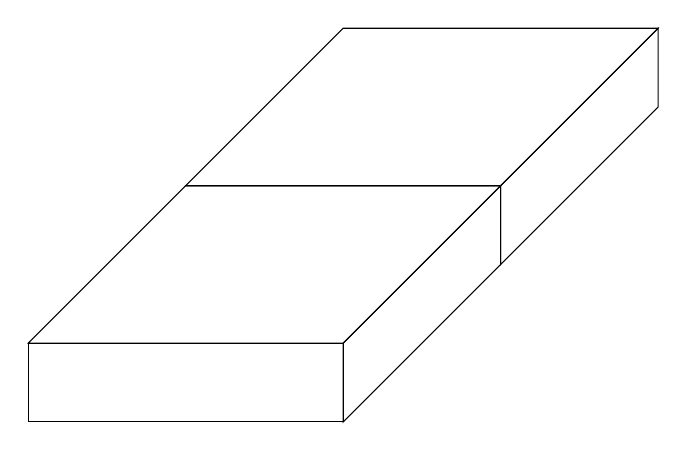
\begin{tikzpicture}[]
            % front
            \draw (0,0) -- (4,0) -- (4,1) -- (0,1) -- cycle;
            % 1st top
            \draw (0,1) -- (2,3) -- (6,3) -- (4,1) -- cycle;
            % 1st boarder
            \draw (4,0) -- (4,1) -- (6,3) -- (6,2) -- cycle;
            % 2nd top
            \draw (2,3) -- (4,5) -- (8,5) -- (6,3) -- cycle;
            % 2nd boarder
            \draw (6,3) -- (8,5) -- (8,4) -- (6,2) -- cycle;
            \end{tikzpicture}
        \end{center}
    \end{figure}
\end{center}


\clearpage
